\documentclass[11pt]{article}
\usepackage[T1]{fontenc}
\usepackage[a4paper,margin=1in]{geometry}
\usepackage{amsmath,amssymb,amsthm}
\usepackage{graphicx}
\usepackage[hidelinks]{hyperref}
\usepackage{microtype}

\newtheorem{theorem}{Theorem}
\newcommand{\E}{\mathbb E}

\setlength{\parindent}{0pt}
\setlength{\parskip}{0.55em}

\title{Chacon Universality Gives a Full Negative Answer\\
to Austin's Weak-Mixing Question}
\author{Literature-implied answer packet\\
Run \texttt{fa\_banach\_001} --- lane 0}
\date{9 August 2026}

\begin{document}
\maketitle

\begin{center}
\fbox{\parbox{0.9\textwidth}{
\textbf{Status: literature-implied answer; full negative resolution.}
The classical Chacon transformation is weakly mixing but cannot be the first
transformation in any divergent bounded double-average example.  The decisive
input is Lesigne--Rittaud--de La Rue's published theorem that Chacon is
universal for weak disjointness.  The short same-space diagonal deduction
below does not appear to have been stated explicitly in the literature.
}}
\end{center}

\section{Source question}

For probability-preserving transformations $S,T$ on the same probability
space and bounded measurable functions $f,g$, consider
\begin{equation}\label{eq:function-average}
 B_N(x):=\frac1N\sum_{n=0}^{N-1}f(S^nx)g(T^nx).
\end{equation}
Austin constructs pairs for which even the integrals of these averages fail to
converge.  His conclusion asks whether every weakly mixing transformation can
appear, up to isomorphism, as $S$ in a nonconvergent example
\cite{Austin}.

\begin{center}

\includegraphics[width=0.96\textwidth]{figures/open_problem_crop.png}
\end{center}

The natural universal reading has a negative answer.  In fact, one classical
weakly mixing system forces convergence for every possible second system and
every pair of bounded observables.

\section{The supporting theorem}

Lesigne, Rittaud, and de La Rue define two systems $(X,\mu,C)$ and
$(Y,\nu,T)$ to be \emph{weakly disjoint} if, for every $f\in L^2(\mu)$ and
$g\in L^2(\nu)$, there are full-measure sets $A\subseteq X$ and $D\subseteq
Y$ such that
\begin{equation}\label{eq:rectangle}
 \frac1N\sum_{n=0}^{N-1} f(C^nx)g(T^ny)
\end{equation}
converges for every $(x,y)\in A\times D$.  A system is called
\emph{universal} if it is weakly disjoint from every dynamical system
\cite[Definition~1]{LRR}.

\begin{center}
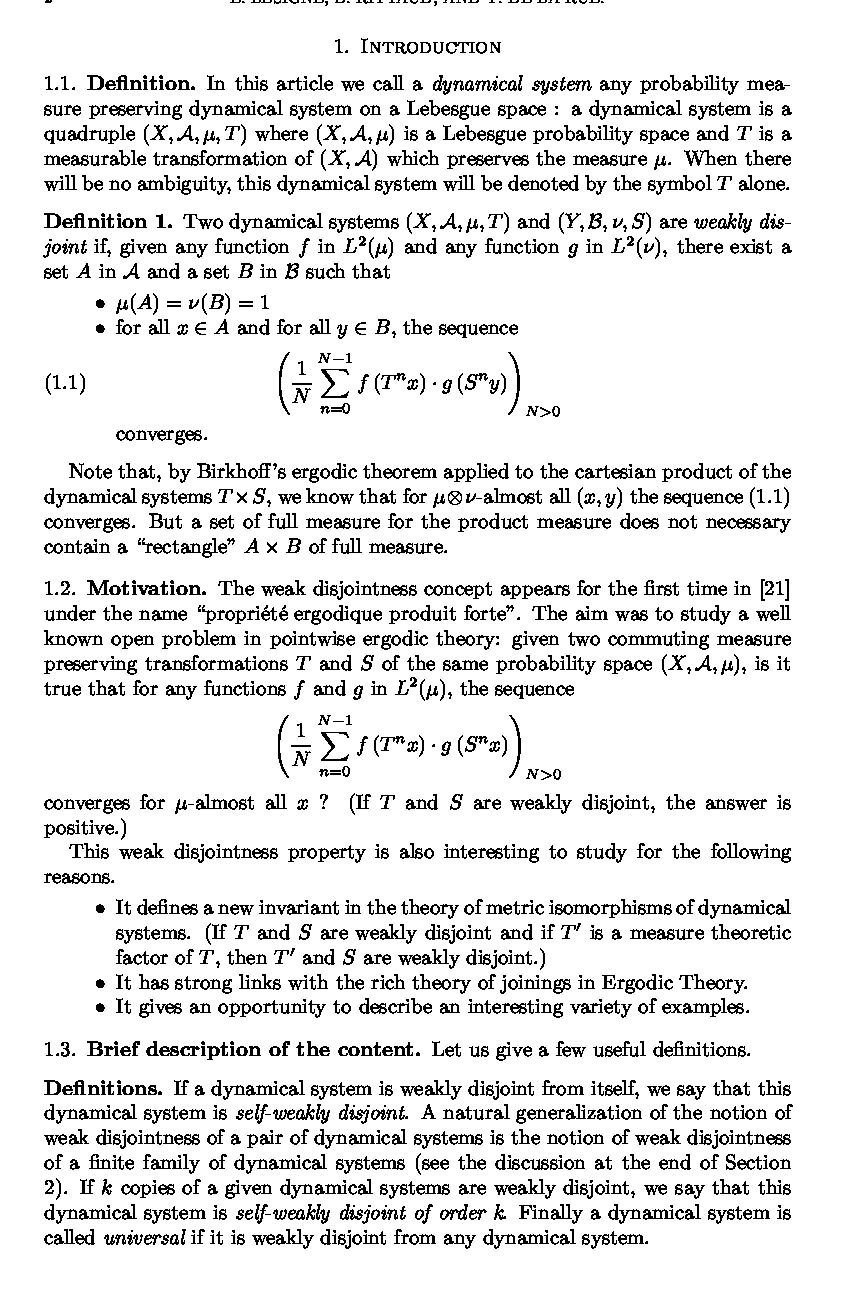
\includegraphics[height=0.63\textheight]{figures/weak_disjointness_definition_crop.png}
\end{center}

The full rectangle in this definition is substantially stronger than ordinary
$\mu\otimes\nu$-almost-everywhere convergence: a product-null diagonal can be
inserted into the rectangle after the two systems are placed on the same
space.

In Section~4.2 the authors first recall that Chacon's transformation is weakly
mixing (but not mixing), and then prove the following statement.

\begin{center}
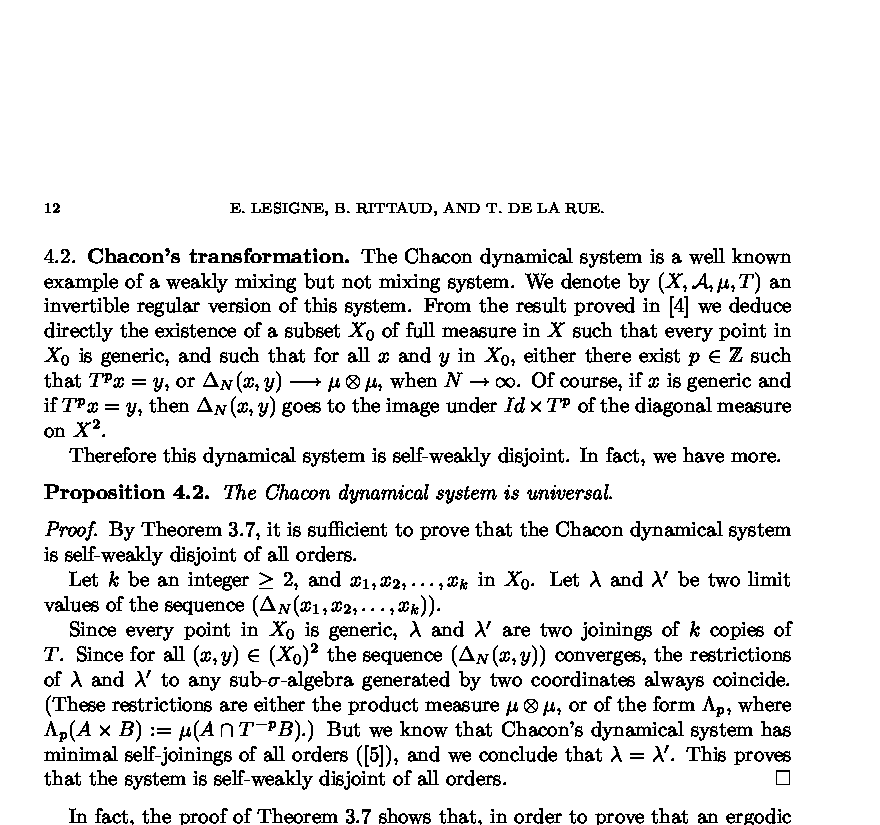
\includegraphics[width=0.92\textwidth]{figures/chacon_universal_crop.png}
\end{center}

Thus Proposition~4.2 of~\cite{LRR} says exactly that Chacon's transformation
is weakly disjoint from every probability-preserving dynamical system.

\section{The diagonal consequence}

\begin{theorem}\label{thm:main}
Let $(X,\mathcal B,\mu,C)$ be an invertible probability-preserving Chacon
system.  For every probability-preserving transformation $T$ of the same
Lebesgue probability space and every $f,g\in L^\infty(\mu)$, the averages
\[
 B_N(x)=\frac1N\sum_{n=0}^{N-1}f(C^nx)g(T^nx)
\]
converge almost everywhere and in $L^p(\mu)$ for every finite $p\geq1$.
Consequently the scalar averages
\[
 I_N=\frac1N\sum_{n=0}^{N-1}
 \int_X f(C^nx)g(T^nx)\,d\mu(x)
\]
converge.  The same conclusions hold when the first system is any system
measurably isomorphic to Chacon's transformation.
\end{theorem}

\begin{proof}
Fix $T,f,g$.  By Proposition~4.2 and Definition~1 of~\cite{LRR}, there are
sets $A,D\in\mathcal B$ with $\mu(A)=\mu(D)=1$ such that the two-point
averages~\eqref{eq:rectangle} converge for every $(x,y)\in A\times D$.
Here the first and second systems act on the same underlying space, so
$E:=A\cap D$ has full measure.  For every $x\in E$, substitute $y=x$ in
\eqref{eq:rectangle}.  This gives exactly the almost-everywhere convergence of
$B_N$.

Let $M=\lVert f\rVert_\infty\lVert g\rVert_\infty$.  Then $|B_N|\leq M$ for
all $N$, and the almost-everywhere limit $B$ also satisfies $|B|\leq M$.
Dominated convergence applied to $|B_N-B|^p$ gives $B_N\to B$ in every finite
$L^p$.  Finally,
\[
 I_N=\int_X B_N\,d\mu \longrightarrow \int_X B\,d\mu,
\]
which proves convergence of the integrated averages.

Weak disjointness is invariant under metric isomorphism
\cite[Introduction]{LRR}.  Equivalently, transporting $T,f,g$ through an
isomorphism reduces an arbitrary copy of Chacon's system to the case just
proved.
\end{proof}

\section{Resolution, provenance, and checks}

Chacon's transformation is weakly mixing, while Theorem~\ref{thm:main} shows
that it cannot appear as $S$ in a nonconvergent example of
\eqref{eq:function-average}.  This answers Austin's universal question
negatively.  It also removes any ambiguity about the convergence mode:
pointwise almost-everywhere convergence, every finite-$L^p$ convergence, and
convergence of the scalar integrals all hold.

The supporting theorem predates Austin's question by more than two decades,
so its authors do not claim to answer that question.  The relation is a direct
agent-identified implication and is therefore recorded as a
\emph{literature-implied answer}, not as a new counterexample or an explicit
later literature answer.

A bounded novelty check through 9 August 2026 searched the run indexes; exact
title, arXiv-id, and question-wording matches; citation and title searches
combining Austin's paper with Chacon, universality, and weak disjointness; and
recent related counterexample papers.  No later source explicitly stating
this corollary was found.  Novelty confidence is intentionally low because the
only substantive dynamical input is the published Proposition~4.2.

\textbf{Human-review recommendation.}  Verify the natural universal reading
of Austin's word ``any'' and the full-rectangle quantifiers in Definition~1.
Once those are fixed, the diagonal substitution and dominated-convergence
steps are immediate.

\begin{thebibliography}{9}

\bibitem{Austin}
T. Austin,
\emph{Non-convergence of some non-commuting double ergodic averages},
Proc. Amer. Math. Soc. \textbf{153} (2025), 1701--1707;
arXiv:\href{https://arxiv.org/abs/2407.08630}{2407.08630}.

\bibitem{LRR}
E. Lesigne, B. Rittaud, and T. de La Rue,
\emph{Weak disjointness of measure preserving dynamical systems},
Ergodic Theory Dynam. Systems \textbf{23} (2003), 1173--1198,
\href{https://doi.org/10.1017/S0143385702001505}{doi:10.1017/S0143385702001505};
HAL:\href{https://hal.science/hal-00017086}{hal-00017086}.

\end{thebibliography}

\end{document}

